\section{Evolutionary Analysis} \label{sec:evolutionary}

Sections \ref{sec:geometric} and \ref{sec:variational} reported how each tag-matching metric induced constraints on tag match affinities and the distribution of mutational outcomes.
We now move on to investigate whether --- and how ---  these geometric and variational properties affect evolution of tag-mediated connectivity in evolutionary scenarios.

We begin with a toy problem, presented in Section \ref{sec:graph-matching}, which allowed us to systematically vary the level of network constraint selected for.
That is, these experiments compared scenarios where individual tags needed to ensure simultaneously tight affinity with several other tags (more constrained) and where individual tags only needed to ensure tight affinity with one other tag (less constrained).
In this toy problem, we define a target connection topology between tagged queries and operands then select for sets of tags that exhibit high-affinity pairings between connected topology elements.

In order to investigate potential consequences of tag-matching metrics in a more generalized, complex domain, we also evolved full-fledged SignalGP programs that mediate module activation via tag matching.

The SignalGP genetic programming representation employs tag-based referencing to facilitate event-driven program execution \citep{lalejini2018evolving}.
In SignalGP, programs are segmented into modules (functions) that may be automatically triggered by exogenously- or endogenously-generated signals.
Tags specify the relationship between signals and signal-handlers (program modules), triggering the module with the closest matching tag to run its linear sequence of instructions.

The SignalGP instruction set, in addition to including traditional GP operations, allows programs to generate arbitrarily-tagged internal signals and broadcast arbitrarily-tagged external signals, and otherwise work in a tag-based context.
SignalGP also supports genetic regulation with promoter and repressor instructions that, when executed, allow programs to adjust how well subsequent signals match with a target function (specified with tag-based referencing) \citep{lalejini2021tag}.
See \cite{lalejini2018evolving} for a more detailed description of SignalGP.

To ensure a broad survey of tag-matching functionality, we performed experiments with a complementary pair of SignalGP problems:
\begin{itemize}
    \item the \textit{Changing-signal Task} (Section \ref{sec:changing-signal}), which is known to select for sparse tag interactions (i.e., low constraint), and
    \item the \textit{Directional-signal Task} (Section \ref{sec:directional-signal}), which is known to select for more dense tag interactions (i.e., high constraint).
\end{itemize}

These experiments used bit flip mutation operators across all metrics.
Note again that generalization to systems with alternate mutation operators (including many with integer-based tags) should be made carefully.

\subsection{Graph-matching Task} \label{sec:graph-matching}

\begin{figure}
% \begin{minipage}{6in}
\begin{center}

\begin{minipage}{0.05\textwidth}
~
\end{minipage}%
\begin{minipage}{0.95\textwidth}
\begin{minipage}{0.05\textwidth}
~
\end{minipage}%
\begin{minipage}{0.95\textwidth}
\centering
\large
\textbf{Mean Degree}
\end{minipage}
\begin{minipage}{0.05\textwidth}
~
\end{minipage}%
\begin{minipage}{0.95\linewidth}
\begin{minipage}{0.5\textwidth}
\centering
\large
1
\end{minipage}%
\begin{minipage}{0.5\textwidth}
\centering
\large
2
\end{minipage}
\end{minipage}
\end{minipage}\\
\vspace{2ex}





\begin{minipage}{0.05\textwidth}
\large
\rotatebox[origin=c]{90}{\textbf{Structure}}
\end{minipage}%
\begin{minipage}{0.95\textwidth}
\begin{minipage}{0.05\linewidth}
\large
\rotatebox[origin=c]{90}{Irregular}
\end{minipage}%
\begin{minipage}{0.95\linewidth}
\begin{subfigure}[b]{0.5\textwidth}
\centering
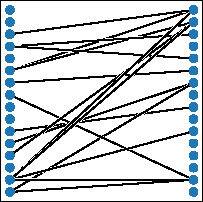
\includegraphics[width=\textwidth]{img/graph_layouts/title=irregular-1+ext=}%
\caption{
Irregular w/ mean degree 1
}
\label{fig:irregular_1}
\end{subfigure}
\begin{subfigure}[b]{0.5\textwidth}
\centering
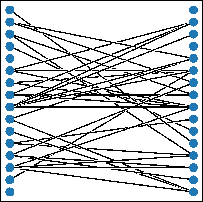
\includegraphics[width=\textwidth]{img/graph_layouts/title=irregular-2+ext=}%
\caption{
Irregular w/ mean degree 2
}
\label{fig:irregular_2}
\label{fig:irregular_degree_2}
\end{subfigure}

\end{minipage}

\vspace{2ex}

\begin{minipage}{\textwidth}

\begin{minipage}{0.05\linewidth}
\large
\rotatebox[origin=c]{90}{Regular}
\end{minipage}%
\begin{minipage}{0.95\linewidth}
\begin{subfigure}[b]{0.5\textwidth}
\centering
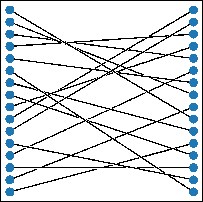
\includegraphics[width=\textwidth]{img/graph_layouts/title=regular-1+ext=}%
\caption{
Regular w/ mean degree 1
}
\label{fig:regular_degree_1}
\label{fig:regular_1}
\end{subfigure}
\begin{subfigure}[b]{0.5\textwidth}
\centering
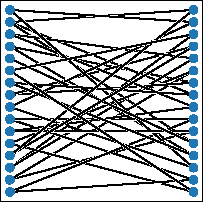
\includegraphics[width=\textwidth]{img/graph_layouts/title=regular-2+ext=}%
\caption{
Regular w/ mean degree 2
}
\label{fig:regular_degree_2}
\label{fig:regular_2}
\end{subfigure}
\end{minipage}
\end{minipage}
\end{minipage}

\caption{
Example target graph layouts used in 32-node graph-matching evolutionary experiments.
Blue dots represent tagged nodes.
Black lines represent selected-for tight affinity relationships.
Layouts differ in total number of selected-for affinities (``mean degree'') and whether selected-for affinities were evenly or randomly distributed between nodes (``structure'').
}
\label{fig:graph_layouts}


\end{center}
% \end{minipage}
\end{figure}

\begin{minipage}{\linewidth}
\begin{center}

\begin{minipage}{\linewidth}
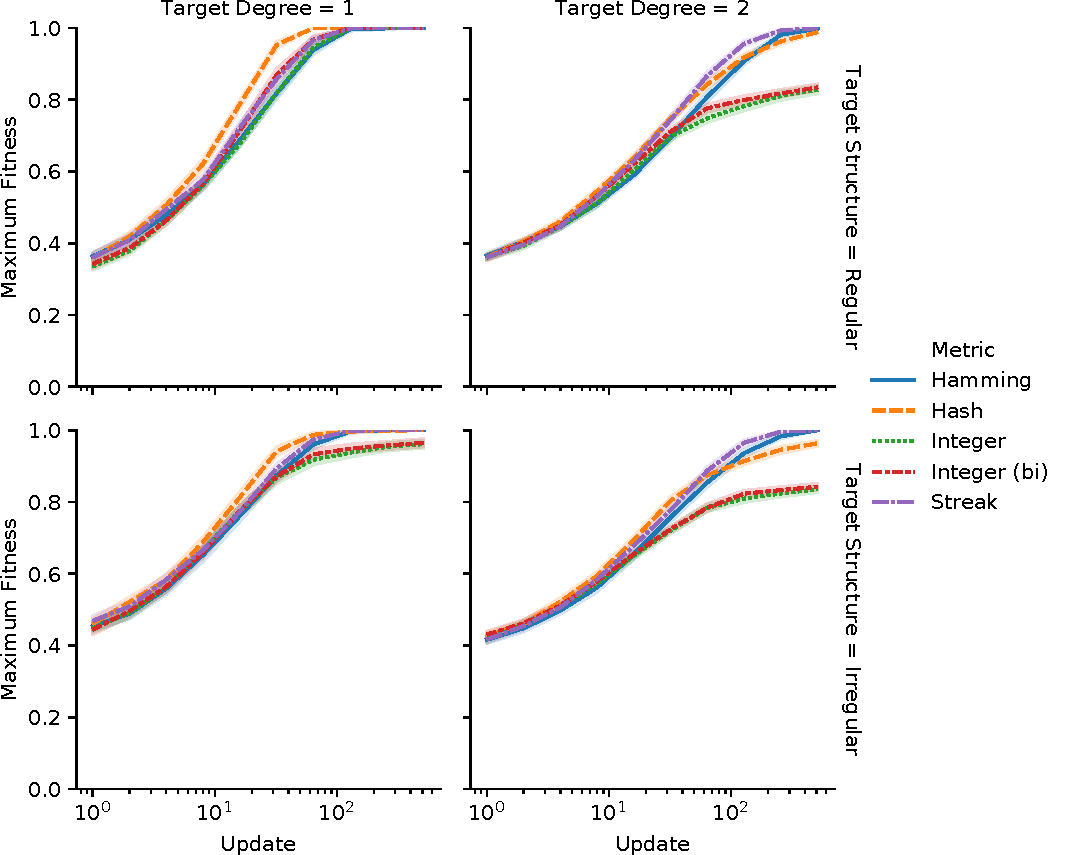
\includegraphics[width=\linewidth]{target_evolve/viz=max-fitness-line+_data_hathash_hash=673d309ab90e91d1+_script_fullcat_hash=fe3ddc711c5abfad+ext=}
\end{minipage}
\begin{minipage}{\linewidth}
\caption{
Maximum fitness by update over replicate runs for each metric's best-performing mutation rate.
Note log-scale x-axes.
Shaded area represents 95\% confidence intervals.
}
\label{fig:evolve_bests}
\end{minipage}
\end{center}
\end{minipage}

\begin{table}[!htbp]
\begin{tabular}{l|l|l|l}
\textbf{Metric}       & \textbf{Target Structure} & \textbf{Target Degree} &  \textbf{\begin{tabular}[c]{@{}l@{}}Best-Performing \\ Per-Genome Bit\\ Mutation Rate\end{tabular}} \\ \hline
Hash                  & Regular                   & 1                      & 0.75                                           \\ \hline
Hash                  & Regular                   & 2                      & 0.75                                           \\ \hline
Hash                  & Irregular                 & 1                      & 1.0                                            \\ \hline
Hash                  & Irregular                 & 2                      & 0.75                                           \\ \hline
Hamming               & Regular                   & 1                      & 4.0                                            \\ \hline
Hamming               & Regular                   & 2                      & 2.0                                            \\ \hline
Hamming               & Irregular                 & 1                      & 4.0                                            \\ \hline
Hamming               & Irregular                 & 2                      & 2.0                                            \\ \hline
Streak                & Regular                   & 1                      & 3.0                                            \\ \hline
Streak                & Regular                   & 2                      & 1.5                                            \\ \hline
Streak                & Irregular                 & 1                      & 4.0                                            \\ \hline
Streak                & Irregular                 & 2                      & 2.0                                            \\ \hline
Integer               & Regular                   & 1                      & 6.0                                            \\ \hline
Integer               & Regular                   & 2                      & 6.0                                            \\ \hline
Integer               & Irregular                 & 1                      & 8.0                                            \\ \hline
Integer               & Irregular                 & 2                      & 8.0                                            \\ \hline
Bidirectional Integer & Regular                   & 1                      & 4.0                                            \\ \hline
Bidirectional Integer & Regular                   & 2                      & 6.0                                            \\ \hline
Bidirectional Integer & Irregular                 & 1                      & 8.0                                            \\ \hline
Bidirectional Integer & Irregular                 & 2                      & 8.0
\end{tabular}

\caption{
Best-performing per-bit mutation rates for 32-vertex graph matching tasks with randomly-initialized genomes.
See Supplementary Figure \ref{fig:evolve_mutsweep} for performance across surveyed mutation rates.
}
\label{tab:evo_graph_mut}

\end{table}


In this experiment, we explored metrics' ability to facilitate evolution of an arbitrary, fixed pattern of tag-matching connectivity.
Genomes in this experiment consisted solely of a set of 32 tags, partitioned evenly as 16 query tags and 16 operand tags.
We used randomly-generated bipartite graphs as a specification for an arbitrary set of desired operands that queries should match to, with each node in the graph corresponding directly to a bitstring tag in the genome.
Figure \ref{fig:graph_layouts} shows example target graph layouts.

To evaluate the fitness of a genome, we harvested its operand tags and placed them into a tag-matching data structure.
This data structure allowed us to match each query tag to its $n$ best-matching operands.
For each query tag, we set the number of collected operand matches $n$ to the outgoing edge count from its corresponding node in the target graph.
So, for example, if a node had three outgoing edges then we would record the three best-matching operands of the corresponding tag.

For the purposes of fitness evaluation, we considered matches within this set equivalent.
So, each query tag had a set of $n$ best-matching operands.
We took that query tag's contribution to fitness as the fraction of its best-matching operands that corresponded to connections on the target bipartite graph; that is, the fraction of best-matching operands with corresponding graph nodes connected by an edge to the query's corresponding graph node.

Along these lines, we took overall fitness as the fraction of best-match tag pairs that correctly corresponded to edges in the target graph.

We controlled the degree of tag-matching constraint imposed by the target graph by manipulating:
\begin{enumerate}
  \item \textit{mean degree} --- the number of edges between queries and operands, and
  \item \textit{structure} --- whether edges were assigned evenly such that all nodes had identical degree (regular structure) or were assigned at random, likely causing some nodes to have high degree (irregular structure).
\end{enumerate}
We tested target graphs with mean degree 1 and 2 and both regular and irregular construction.

Irregular, degree 2 graphs imposed the most tag-matching constraint.
High-degree nodes in these graphs were strongly constrained by many simultaneous connection criteria.
Figure \ref{fig:irregular_degree_2} shows an example irregular, degree 2 graph.

Regular, degree 1 graphs imposed the least tag-matching constraint.
Figure \ref{fig:regular_degree_1} shows an example regular, degree 1 graph.

For each target graph configuration, we surveyed each metric's performance over ten per-bit mutation rates ranging from 0.75 expected bit mutations per genome to 16.0 expected bit mutations per genome.
For each combination of metric and target graph configuration, we report results from the most favorable mutation rate (as defined by sum population-maximum fitness across evolutionary generations).%
\footnote{%
Supplementary Figure \ref{fig:evolve_mutsweep} shows the rate each metric's rate of adaptive evolution across surveyed mutation rates for each target graph configurations.
All treatments' optimal mutation rates fall within the range of mutation rates surveyed, except for the hash metric on the regular target graphs.
In this case, peak performance was observed on the lowest sampled mutation rate.
}
Table \ref{fig:evo_graph_mut} provides the best-performing mutation rate for each metric across target graph configurations.
Best-performing mutation rates varied greatly, ranging from as low as 0.75 expected mutations per genome for the hash metric to as high as 8.0 for the integer metrics.
The Hamming and streak metrics intermediate best-performing mutation rates between 1.5 and 4.0 expected mutations per genome.

We ran 100 replicate 512-generation evolutionary runs for each mutation rate/target graph/tag-matching metric combination.
These runs had a well-mixed population of size 500 and used tournament selection with tournament size 7.
Figure \ref{fig:evolve_bests} plots population-maximum fitness over the course of these evolutionary runs.
We performed the same evolutionary experiment with larger 64-node target graphs and observed qualitatively similar results (Supplementary Figures \ref{fig:evolve_bests64} and \ref{fig:evolve_big_mutsweep}).

\subsubsection{Hash Metric}

Surprisingly, the hash metric enables faster adaptive evolution than all other metrics on the least-constrained target graph (Figure \ref{fig:evolve_bests}; non-overlapping 95\% CI).
On more-constrained target graphs with mean degree 2, the hash metric's advantage in rapid adaptive evolution disappears.
In fact, on the most-constrained target graph (irregular structure with mean degree 2) the hash metric yields significantly lower-quality solutions at the end of evolutionary runs than the streak and Hamming metrics (Figure \ref{fig:evolve_bests}; non-overlapping 95\% CI).

\subsubsection{Hamming and Streak Metrics}

The streak metric facilitates slightly faster adaptive evolution than the Hamming metric, especially on mean degree 2 regularly configured target graphs (Figure \ref{fig:evolve_bests}; non-overlapping 95\% CI).

\subsubsection{Integer Metrics}

The integer and bidirectional integer metrics successfully match the least-constrained target graph (regular structure with mean degree 1) but yield lower-quality solutions than other metrics on more constrained target graphs (Figure \ref{fig:evolve_bests}; non-overlapping 95\% CI).


\subsection{Changing-signal Task} \label{sec:changing-signal}

\begin{figure}[!htbp]
\centering
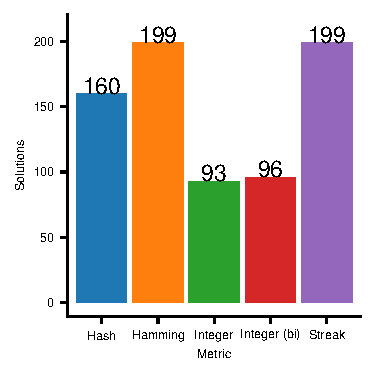
\includegraphics[width=0.75\linewidth]{img/gp_results/panel-cst-sols.pdf}

\caption{
Evolutionary performance of tag-matching metrics on the changing signals task.
Shows the numbers of replicates out of 200 that produced a complete task solution to the changing-signal and directional-signal task respectively.
Results for each metrics' best-performing mutation rate are reported.
}

\label{fig:cst-sols}

\end{figure}


The changing-signal task requires SignalGP programs to express a certain, distinct response to each of $K$ environmental signals.
Environmental signals correspond to a unique tagged event.
Programs express a response by executing one of $K$ response instructions.
Successful programs can ``hardcode'' each response to the appropriate environmental signal by ensuring that each tagged environmental signal best matches the function containing its correct response.
Thus, in this experiment SignalGP module tags are minimally constrained --- each needs to only match with a single environmental signal.

During evaluation, we afford programs 64 virtual CPU cycles to express the appropriate response after receiving a signal.
Once a program expresses a response or the allotted time expires, we reset the program's virtual hardware (resetting all executing threads and thread-local memory), and the environment produces the next signal.
Evaluation continues until the program correctly responds to each of the $K$ environmental signals or until the program expresses an incorrect response.
During each evaluation, programs experience environmental signals in a random order; thus, the correct \textit{order} of responses will vary and cannot be hardcoded.

For each tag-matching metric, we evolved 200 replicate populations (each with a unique random number seed) of 500 asexually reproducing programs in an eight-signal environment for 100 generations.
We identified the most performant per-bit tag mutation rates (from a range of possible mutation rates) for each metric on the changing-signal task:
\begin{itemize}
    \item 0.01 for the Hamming and streak metrics,
    \item 0.002 for the hash metric, and
    \item 0.02 for the integer and bidirectional integer metrics.
\end{itemize}
Aside from tag mutation rate, the overall configuration used for each metric was identical.

We limited tag variation in offspring to tag mutation operators (bit flips) by initializing populations with a common ancestor program in which all tags were identical and by disallowing mutations that would insert instructions with random tags.
Supplemental Section \ref{sec:gpsupplement} gives the full configuration details for this experiment, including a guide for replication.

% \begin{figure*}
  \begin{center}

  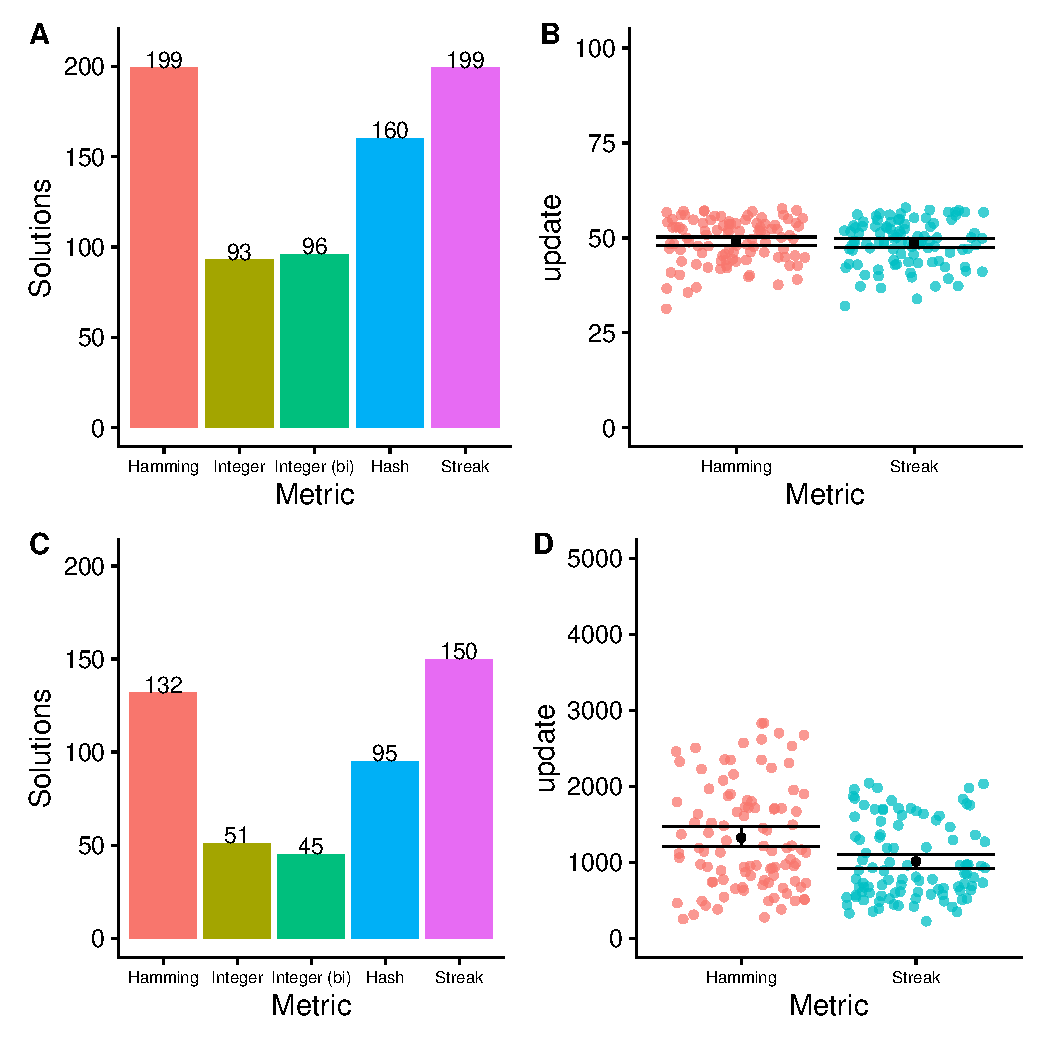
\includegraphics[width=\columnwidth]{img/gp_results/gp_results_panel}
  \caption{
  Todo - caption. A, B are changing-signal task; C, D are directional signal task.
  }
  \label{fig:gp_results}

  \end{center}
  \end{figure*}

Figure \ref{fig:cst-sols} gives the number of replicates that produced a successful SignalGP program (i.e., capable of achieving maximum fitness) for each tag-matching metric on the changing-signal task.
We compared the number of successful replicates across metrics using a pairwise Fisher's exact test with a Holm correction for multiple comparisons.

\subsubsection{Hash Metric}

The hash metric significantly outperformed both integer metrics ($p < 4\times10^{-10}$).

We suspect that the hash metric performed well because it maximizes generation of phenotypic variation (i.e., signal-function relationships).
Even a single bit flip in a tag is likely to completely re-order which other tags it best matches with.
The capacity to quickly generate large amounts of phenotypic variation allows evolution to explore large swaths of the fitness landscape from generation to generation, which is particularly useful in this low-constraint problem.
However, as evidenced by better performance of the Hamming and streak metrics, this capacity to generate phenotypic variation trades off with tag-matching robustness --- under this metric, a single bit mutation may also scramble established relationships with other tags.

\subsubsection{Hamming and Streak Metrics}

The Hamming and streak metrics performed significantly better than all other metrics ($p < 5\times10^{-11}$); however, there was no significant difference in performance between the Hamming and streak metrics.
To assess whether the streak metric produced solutions in fewer generations than the Hamming metric, we ran 200 new replicates of each condition until 100 replicates produced a solution and recorded the number of generations that elapsed (Supplementary Figure \ref{fig:cst-times}).
We found no difference in generations elapsed between the Hamming and streak metrics.

\subsubsection{Integer Metrics}

Among surveyed tag-match metrics, the integer metrics performed worst.
We observed no adaptive difference  between the integer and bidirectional integer metrics.

\subsection{Directional-signal Task} \label{sec:directional-signal}

\begin{figure}

\begin{subfigure}[b]{\linewidth}
\centering
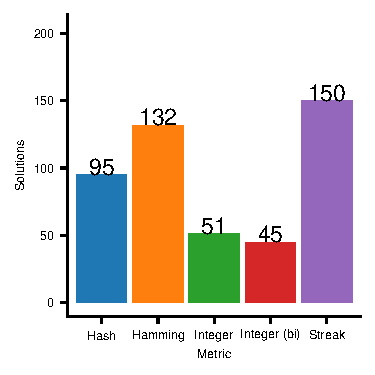
\includegraphics[width=0.75\linewidth]{img/gp_results/panel-dst-sols.pdf}%
\caption{
Numbers of replicates out of 200 that produced a complete solution to the directional-signal task.}
\label{fig:dst-sols}
\end{subfigure}
\begin{subfigure}[b]{\linewidth}
\centering
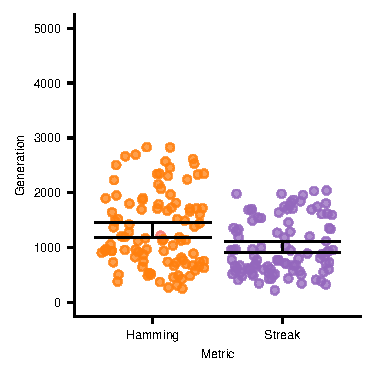
\includegraphics[width=0.75\textwidth]{img/gp_results/panel-dst-times.pdf}%
\caption{
Generations to solution for the first 100 replicates out of 200 to produce a complete solution to the directional-signal task.
Error bars indicate bootstrapped 95\% confidence intervals.
}
\label{fig:dst-times}
\end{subfigure}

\label{fig:gp_results}

\caption{
Evolutionary performance of tag-matching metrics on the directional signals.
All show each metrics' best-performing mutation rate.
}

\label{fig:evo_directional_signal}
\end{figure}

As in the changing-signal task, the directional-signal task requires that programs respond to a sequence of environmental cues.
In the directional-signal task, however, the correct response to signal depends on the history previously experienced signals.
In the directional-signal task, there are two possible environmental signals --- a ``forward signal'' and a ``backward signal'' (each with a distinct tag) ---  and a cycle of four possible responses.
If a program receives a forward-signal, it should express the next response in the cycle.
If the program receives, a backward-signal, it should express the previous response in the cycle.
For example, if response three is currently required, a subsequent forward signal indicates that response four is required next, while a backward signal would instead indicate that response-two is required next.
Because the appropriate response to both the backward and forward signals change over time, successful programs must regulate which functions these signals trigger (rather than hardcode each response to a particular signal).

SignalGP module tags are more constrained than in the changing-signal task, potentially needing to match to queries by genetic regulation instructions in addition to \textit{several} tagged events (e.g., environmental signals or internally-generated signals) depending on internal regulatory state.
Indeed, in other work, we have observed that the directional signal task yields significantly more interconnected regulatory networks than the changing signal task \citep{lalejini_tag-based_2021}.

% Evaluation overview
We evaluated programs on all possible four-signal sequences of forward and backward signals (sixteen total).
For each program, we evaluated each sequence of signals independently, and a program's fitness was taken as its aggregate performance.
Otherwise, evaluation on a single sequence of signals mirrors that of the changing signal task.

% Experiment overview
We used an identical experimental design for the directional-signal task as in the changing signal task.
However, we evolved programs for 5,000 generations (instead of 100) and re-parameterized each metric's tag mutation rate:
\begin{itemize}
\item 0.001 for the Hamming and hash metrics,
\item 0.002 for the integer and streak metrics, and
\item 0.0001 for the bidirectional integer metric.
\end{itemize}
Full configuration details for this experiment, including a guide for replication, appears in Supplemental Section \ref{sec:gpsupplement}.

% Results
Figure \ref{fig:dst-sols} gives the number of replicates that produced a successful SignalGP program for each tag-matching metric on the directional-signal task.

\subsubsection{Hamming and Streak Metrics}

Again, the Hamming and streak metrics performed significantly better than all other metrics (Fisher's exact with a Holm correction for multiple comparisons, $p < 0.0008$).
We observed no significant difference in solution count between the Hamming and streak metrics, however.

As in the changing-signal task, we assessed whether the streak metric produced solutions in fewer generations than the Hamming metric, running 200 new replicates of each condition until 100 replicates produced a solution and recorded the number of generations that elapsed (Figure \ref{fig:dst-times}).
Among this subset of replicates, we found significantly faster generations-to-solution under the streak metric compared to the Hamming metric (Wilcoxon rank-sum test, $p < 0.0016$).

\subsubsection{Integer and Hash Metrics}

As in the changing-signal task, we observed no difference in success between the integer and bidirectional integer metrics on both the changing- and directional-signal tasks.
Again, the hash metric outperformed both the integer metrics ($p < 3\times10^{-5}$).
%Intuitively, the Hash metric maximizes the amount of phenotypic variation (\textit{i.e.}, signal-function relationships) that can be generated by mutating a given genotype --- a single bit flip in a tag is likely to completely re-order which other tags it best matches with.
%The capacity to quickly generate large amounts of phenotypic variation allows evolution to explore a large swaths of the fitness landscape from generation to generation.
%However, this capacity to generate phenotypic variation trades off with tag-matching robustness --- a single mutation may also scramble any established relationships with other tags.
%Further, of each of the metrics we explored, the Hash metric is the most susceptible to mutational meltdowns at high mutation rates.

%[Statement about consistency with expectations based on previous tag-matching experiments].
% - Appears to be consistent with results from graph matching evolution experiment. Needs confirmation, though.
% - Interesting that these two metrics seem to have fairly different geometric properties (because wrap-around vs no wrap-around), but have fairly similar variational properties.
% - For GP problems here, wrap-around vs no wrap around seems to not make a difference.


% TODO - double check that result in analyses
% [Statement about consistency with expectations based on previous tag-matching experiments].
% Seems largely consistent with mean-degree-2 results (for later updates) in graph matching evolution experiment.
% More work to be done, but these data indicate that streak metric can be used for best/consistent performance in GP.
